\newpage
\section{Die Landkreise und Regierungsbezirke sortiert nach dem Gemeindeschlüssel}
\autoref{sec:Vorgehensweise:Datendarstellung:Allgemeine Daten der Gebiete} folgend, wird in diesem Abschnitt die räumliche Verteilung der Gemeindeschlüssel dargestellt.
In \autoref{fig:distribution_AdmUnitId} sind die Landkreise und Regierungsbezirke entsprechend der lexikographischen Ordnung der Gemeindeschlüssel eingefärbt, wie sie in  \autoref{sec:Grundlagen:lexikographisch} beschrieben ist. In der Abbildung lässt sich der in \autoref{sec:Vorgehensweise:Datendarstellung:Allgemeine Daten der Gebiete} angesprochene grobe Nord-Süd- und Ost-West-Verlauf erkennen. Das Saarland bildet hierbei leider eine Ausnahme, wie auch in der nach Gemeindeschlüssel sortierten Listen der Landkreise und den Regierungsbezirken in \autoref{tab:counties_by_admunitid} und \autoref{tab:districts_by_pop_density} sichtbar.
\begin{figure}[H]
    \centering
    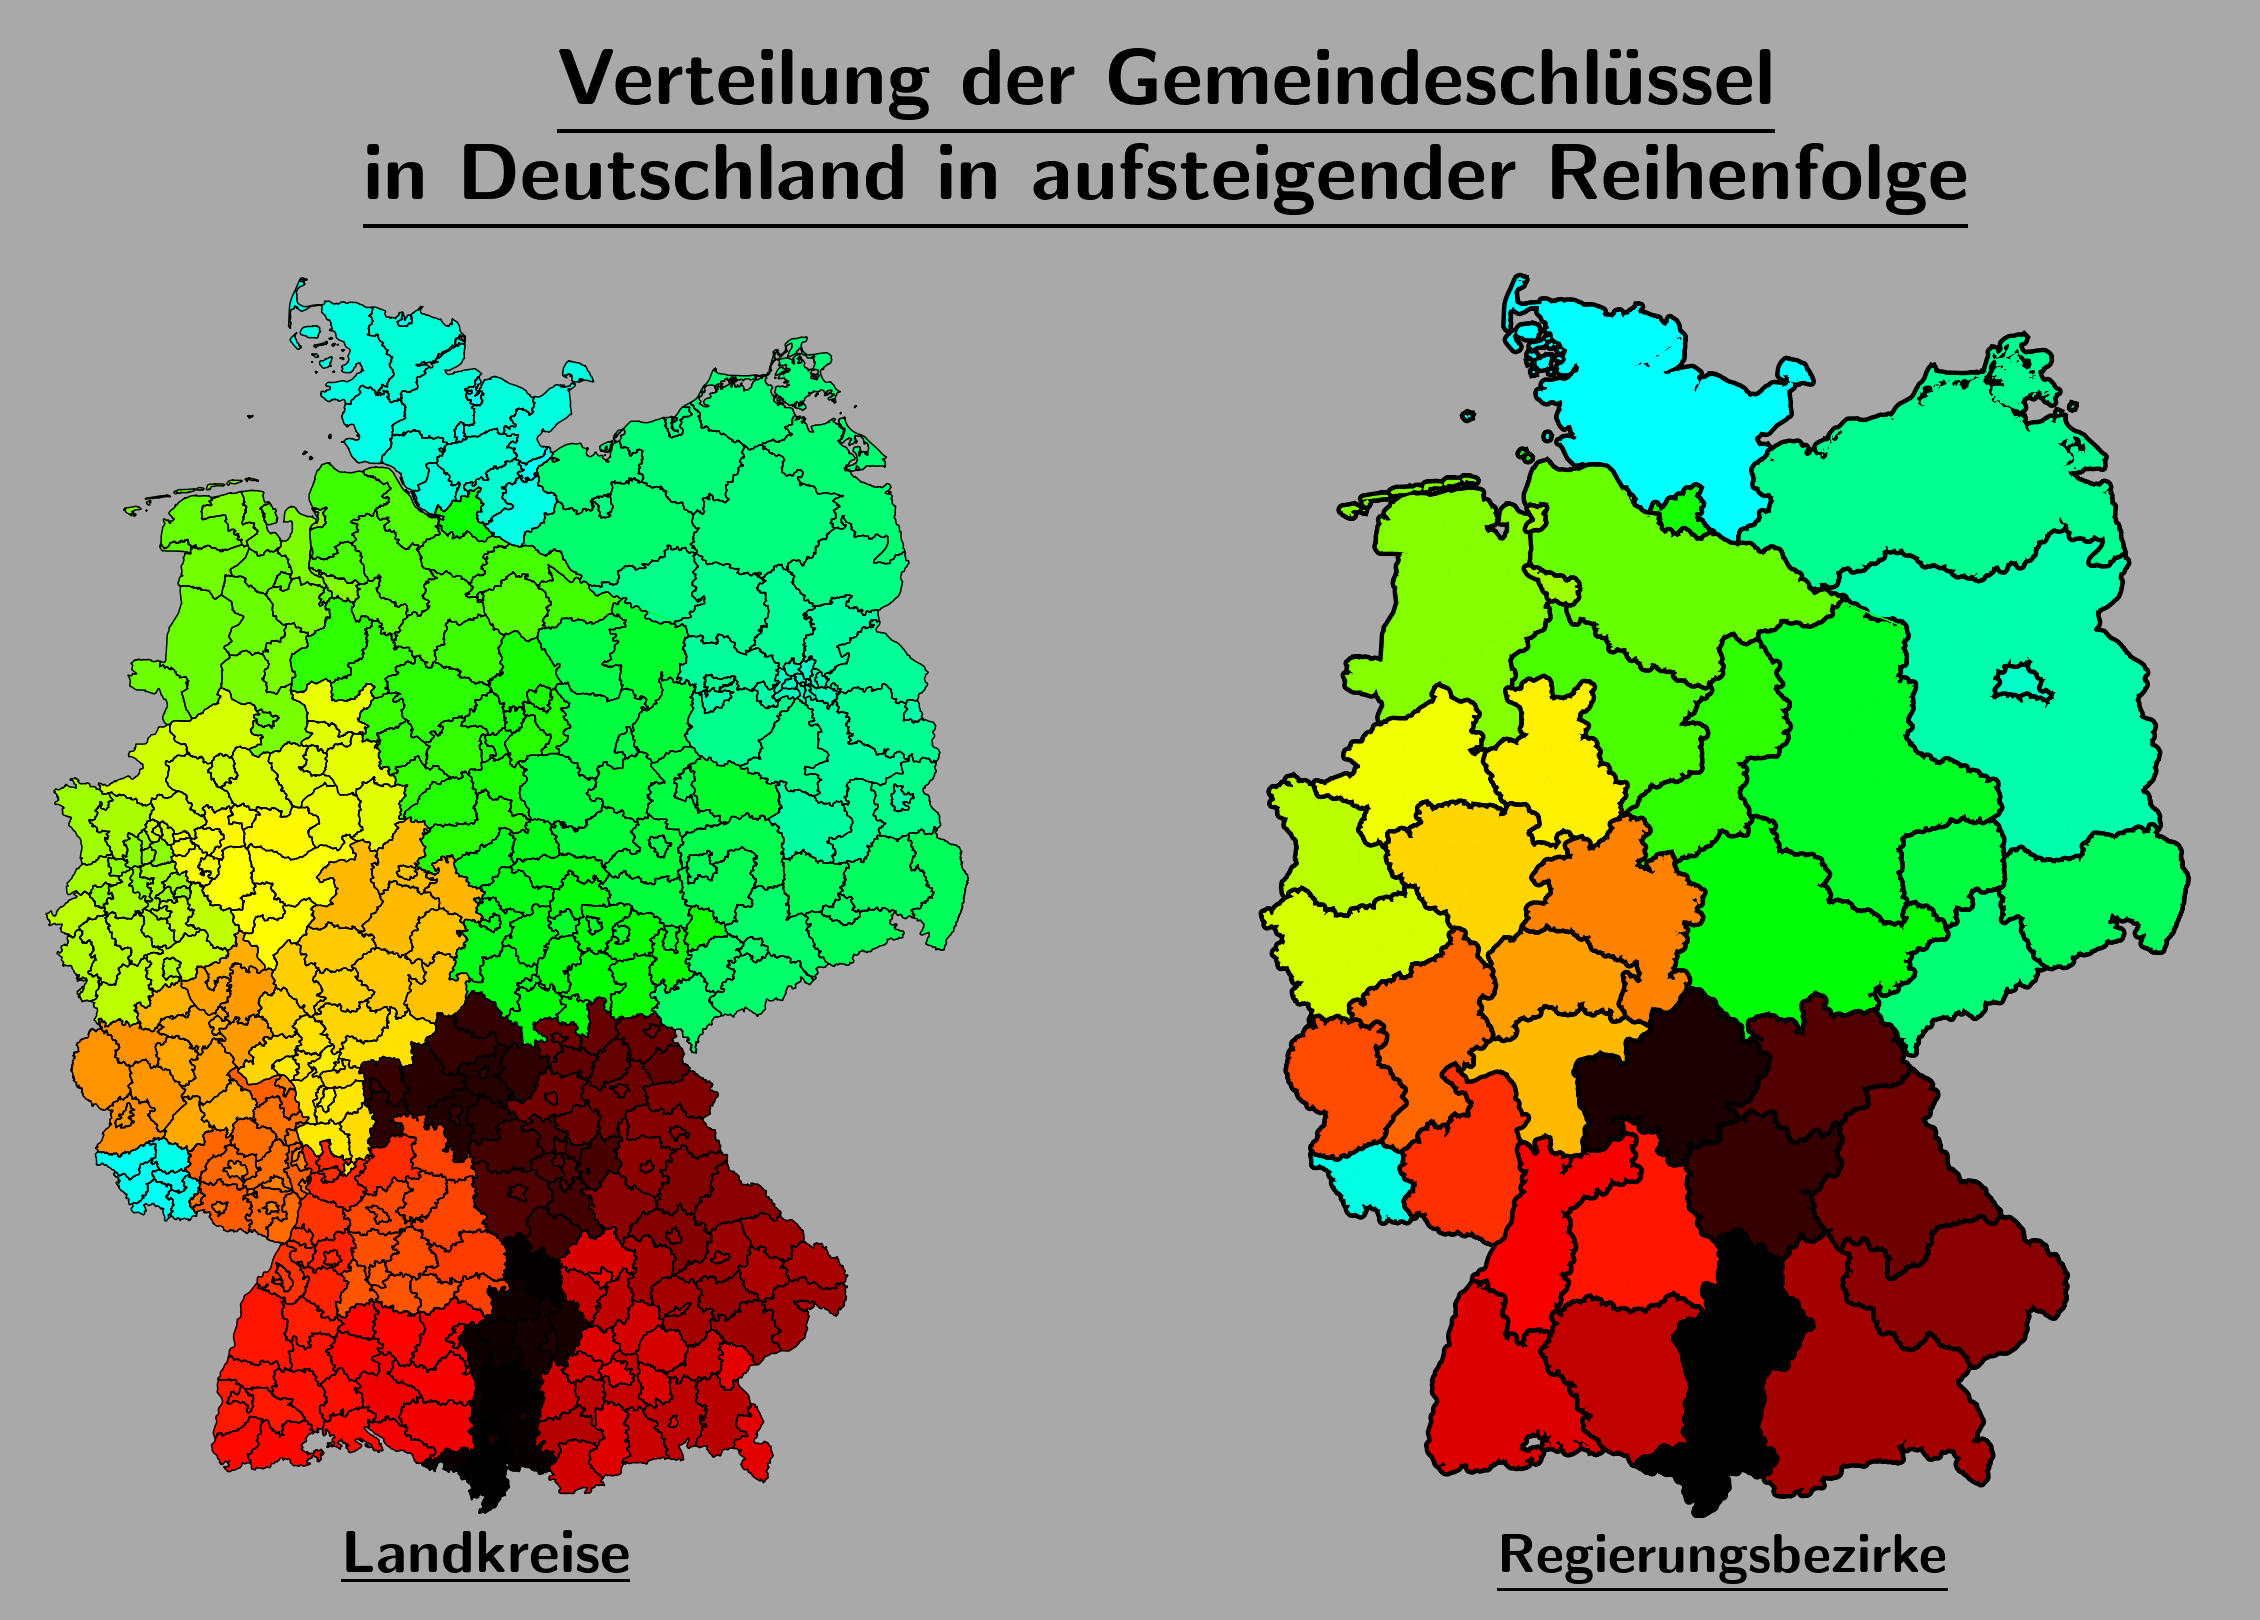
\includegraphics[width = \textwidth]{figures/Ergebnisse/districts_and_counties_by_AdmUnitID.png}
    \caption{Die Landkreise und Regierungsbezirke eingefärbt nach der lexikographischen Größe ihres Gemeindeschlüssels.}
    \label{fig:distribution_AdmUnitId}
\end{figure}